% CDM RAG API - technical walkthrough (exactly 3 slides, no title slide)
% Compile:  pdflatex presentation.tex   (run twice)   or   latexmk -pdf presentation.tex
\documentclass[aspectratio=169,10pt]{beamer}

\usepackage[T1]{fontenc}
\usepackage[utf8]{inputenc}
\usepackage{lmodern}
\usepackage{tikz}
\usetikzlibrary{arrows.meta,positioning}

\usetheme{default}
\setbeamertemplate{navigation symbols}{}
\setbeamertemplate{footline}{%
  \hfill\scriptsize\color{gray}CDM RAG API \quad \insertframenumber/3\hspace*{2mm}\vspace*{1.5mm}}
\definecolor{accent}{RGB}{0,90,160}
\definecolor{soft}{RGB}{232,240,248}
\definecolor{warn}{RGB}{170,60,0}
\setbeamercolor{frametitle}{fg=accent}
\setbeamerfont{frametitle}{series=\bfseries,size=\large}
\setbeamercolor{itemize item}{fg=accent}
\setbeamertemplate{itemize item}{\small$\bullet$}
\setbeamertemplate{itemize subitem}{\scriptsize$-$}
\setbeamerfont{itemize/enumerate subbody}{size=\scriptsize}

\newcommand{\code}[1]{\texttt{#1}}

\tikzset{
  box/.style={draw=accent, fill=soft, rounded corners=2pt, align=center,
              font=\scriptsize, minimum height=10mm, inner sep=3pt, text width=#1},
  box/.default=20mm,
  flow/.style={-{Stealth[length=2mm]}, thick, accent},
  note/.style={font=\tiny, text=gray, align=center},
}

\begin{document}

% ---------------------------------------------------------------------------
\begin{frame}{1 \;|\; Architecture \& data flow}
\centering
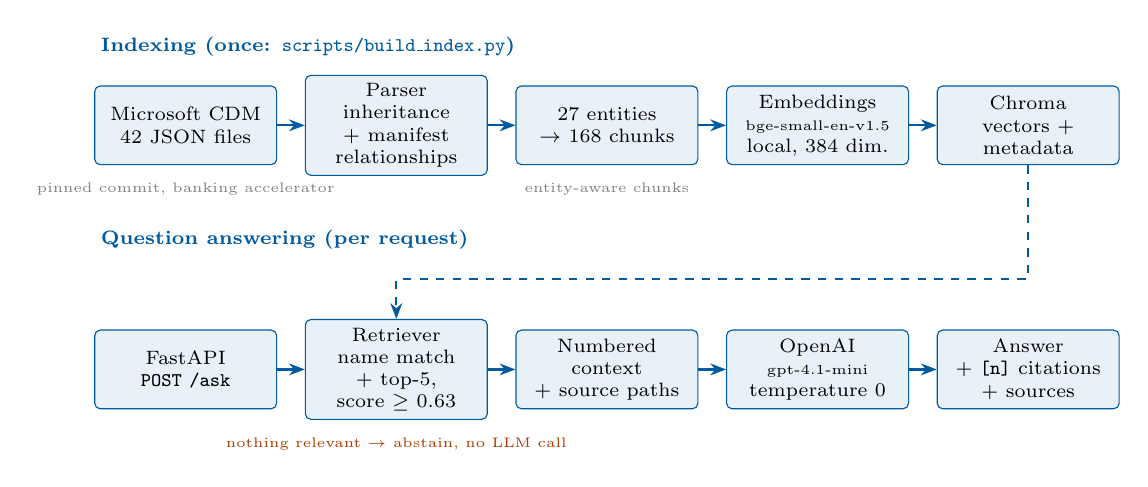
\begin{tikzpicture}[node distance=3.5mm]
  % offline indexing
  \node[font=\scriptsize\bfseries, text=accent, anchor=west] (t1) at (-0.6,1.6) {Indexing (once: \code{scripts/build\_index.py})};
  \node[box=21mm] (cdm) at (0.6,0.6) {Microsoft CDM\\ 42 JSON files};
  \node[box=21mm, right=of cdm] (parse) {Parser\\ inheritance + manifest relationships};
  \node[box=21mm, right=of parse] (ent) {27 entities\\ $\rightarrow$ 168 chunks};
  \node[box=21mm, right=of ent] (emb) {Embeddings\\ \mbox{\tiny bge-small-en-v1.5}\\ local, 384 dim.};
  \node[box=21mm, right=of emb] (db) {Chroma\\ vectors + metadata};
  \draw[flow] (cdm) -- (parse);
  \draw[flow] (parse) -- (ent);
  \draw[flow] (ent) -- (emb);
  \draw[flow] (emb) -- (db);
  \node[note, below=1mm of cdm] {pinned commit, banking accelerator};
  \node[note, below=1mm of ent] {entity-aware chunks};

  % online query
  \node[font=\scriptsize\bfseries, text=accent, anchor=west] (t2) at (-0.6,-0.85) {Question answering (per request)};
  \node[box=21mm] (api) at (0.6,-2.5) {FastAPI\\ \code{POST /ask}};
  \node[box=21mm, right=of api] (ret) {Retriever\\ name match + top-5, score $\ge$ 0.63};
  \node[box=21mm, right=of ret] (ctx) {Numbered context\\ + source paths};
  \node[box=21mm, right=of ctx] (llm) {OpenAI\\ \mbox{\tiny gpt-4.1-mini}\\ temperature 0};
  \node[box=21mm, right=of llm] (ans) {Answer\\ + \code{[n]} citations + sources};
  \draw[flow] (api) -- (ret);
  \draw[flow] (ret) -- (ctx);
  \draw[flow] (ctx) -- (llm);
  \draw[flow] (llm) -- (ans);
  % dashed: the retriever reads the index; routed below the "Question answering" label
  \draw[flow, dashed] (db.south) |- (5.2,-1.35) -| (ret.north);
  \node[note, below=1mm of ret, text=warn] {nothing relevant $\rightarrow$ abstain, no LLM call};
\end{tikzpicture}

\vspace{1mm}
\begin{columns}[T]
\begin{column}{0.48\textwidth}
\scriptsize
\begin{itemize}
  \item Python 3.12, FastAPI, Pydantic, sentence-transformers, Chroma, OpenAI SDK
  \item Plain Python pipeline (no LangChain): each step is one small module
\end{itemize}
\end{column}
\begin{column}{0.48\textwidth}
\scriptsize
\begin{itemize}
  \item Endpoints: \code{/ask}, \code{/retrieve} (no LLM), \code{/health}, Swagger \code{/docs}
  \item Docker: model and index built into the image, key only at runtime
\end{itemize}
\end{column}
\end{columns}
\end{frame}

% ---------------------------------------------------------------------------
\begin{frame}{2 \;|\; Embedding \& retrieval strategy}
\begin{columns}[T]
\begin{column}{0.49\textwidth}
\small\textbf{\color{accent}Documents: one entity = one unit of meaning}
\scriptsize
\begin{itemize}
  \item Scope: \emph{banking accelerator} (24 entities) + 3 common entities; parents merged (Account: 4 files, 120 attributes)
  \item Chunks follow entity boundaries, not fixed token windows:
  \begin{itemize}
    \item \code{overview}: description, inheritance, outgoing relationships
    \item \code{referenced\_by}: incoming relationships
    \item \code{attributes}: 12 per chunk, each starts with \code{Entity: <name>}
  \end{itemize}
  \item Split because whole entities reached 700 tokens (limit 512); largest chunk now 416
\end{itemize}

\vspace{1mm}
\small\textbf{\color{accent}Embedding model and vector store}
\scriptsize
\begin{itemize}
  \item \code{BAAI/bge-small-en-v1.5}: local, CPU, 384 dim., 512-token input
  \item Chroma: vectors, text and metadata together; cosine; persistent on disk
\end{itemize}
\end{column}

\begin{column}{0.49\textwidth}
\small\textbf{\color{accent}Retrieval per question}
\scriptsize
\begin{enumerate}
  \item \textbf{Entity-name match} (``financial product'' = \code{FinancialProduct}):\\
        always add \code{overview} + \code{referenced\_by} of up to 3 named entities
  \item \textbf{Vector search}: top-$k$ = 5 (+ BGE query instruction)
  \item \textbf{Threshold}: keep cosine score $\ge$ 0.63
  \item Merge without duplicates; empty $\rightarrow$ abstain
\end{enumerate}

\vspace{1mm}
\small\textbf{\color{accent}Why these choices (measured)}
\scriptsize
\begin{itemize}
  \item ``How does a Contact relate to an Account?'': vector search alone returned
        only attribute chunks $\rightarrow$ name matching adds the relationship chunks
  \item Top-1 scores: in-scope $\ge$ 0.66, off-topic $\le$ 0.61 $\rightarrow$ threshold 0.63
  \item Evaluation script: 17/18 checks.\\
        Miss: ``assets pledged to secure a loan'' does not find \code{Collateral}
\end{itemize}
\end{column}
\end{columns}
\end{frame}

% ---------------------------------------------------------------------------
\begin{frame}{3 \;|\; Relationships, reliability \& testing}
\begin{columns}[T]
\begin{column}{0.32\textwidth}
\small\textbf{\color{accent}Relationships}
\scriptsize
\begin{itemize}
  \item Source: explicit \code{relationships} list in the official manifests
  \item Stored per entity: outgoing + incoming
  \item Written as text:\\ \code{Contact.parentCustomerId}\\ \hspace*{2mm}$\rightarrow$ \code{Account.accountId}
  \item Audit links (\code{createdBy}, \code{ownerId}) summarized separately
  \item Named entities: both sides retrieved
  \item No graph DB: 27 entities, one-hop questions
\end{itemize}
\end{column}

\begin{column}{0.33\textwidth}
\small\textbf{\color{accent}Reducing hallucinations}
\scriptsize
\begin{itemize}
  \item No relevant chunk $\rightarrow$ fixed answer, \textbf{no LLM call}
  \item Prompt: only the \code{<context>}; no invented entities, attributes or links;
        fixed sentence if context is insufficient; say when lists are partial
  \item Temperature 0, numbered blocks, \code{[n]} citations, source file paths
  \item Checked: all 28 attributes and 5 relationships in demo answers exist in the data
  \item Example: no direct Contact $\rightarrow$ Organization link $\rightarrow$ answer says so
\end{itemize}
\end{column}

\begin{column}{0.32\textwidth}
\small\textbf{\color{accent}Testing}
\scriptsize
\begin{itemize}
  \item 58 pytest tests, $\sim$6\,s, no network, no OpenAI
  \item Fakes: keyword embedder, in-memory Chroma, fake OpenAI client
  \item Parser, chunks, retrieval (name match, threshold, off-topic), RAG service, API (422/503)
  \item Retrieval evaluation on the real index
\end{itemize}

\vspace{1mm}
\small\textbf{\color{warn}Limitations}
\scriptsize
\begin{itemize}
  \item Small scope; no reranker or keyword search
  \item Attribute lists can be partial
  \item Threshold from a small sample
  \item Depends on OpenAI; no auth
\end{itemize}
\end{column}
\end{columns}
\end{frame}

\end{document}
